\section{Introduction}
\label{sec:intro}

A stepper is a programming tool that can display the intermediate states that arises when evaluating an expression.Steppers promise to ease debugging and learning. \citet{findler_drscheme_2002} developed a stepper with error detection. However, it can only provide feedback for complete programs that don't have missing pieces. \Hazel, a pure functional programming language environment developed by \citet{HazelnutPOPL}, assigns semantic meaning to incomplete programs. It contains a special form called hole indicating missing expressions. In this paper, we want to develop an interactive stepper for \Hazel. Take the following programs as examples:

\begin{figure}[htbp]
  \centering
  \begin{subfigure}[b]{0.3\textwidth}
      \centering
      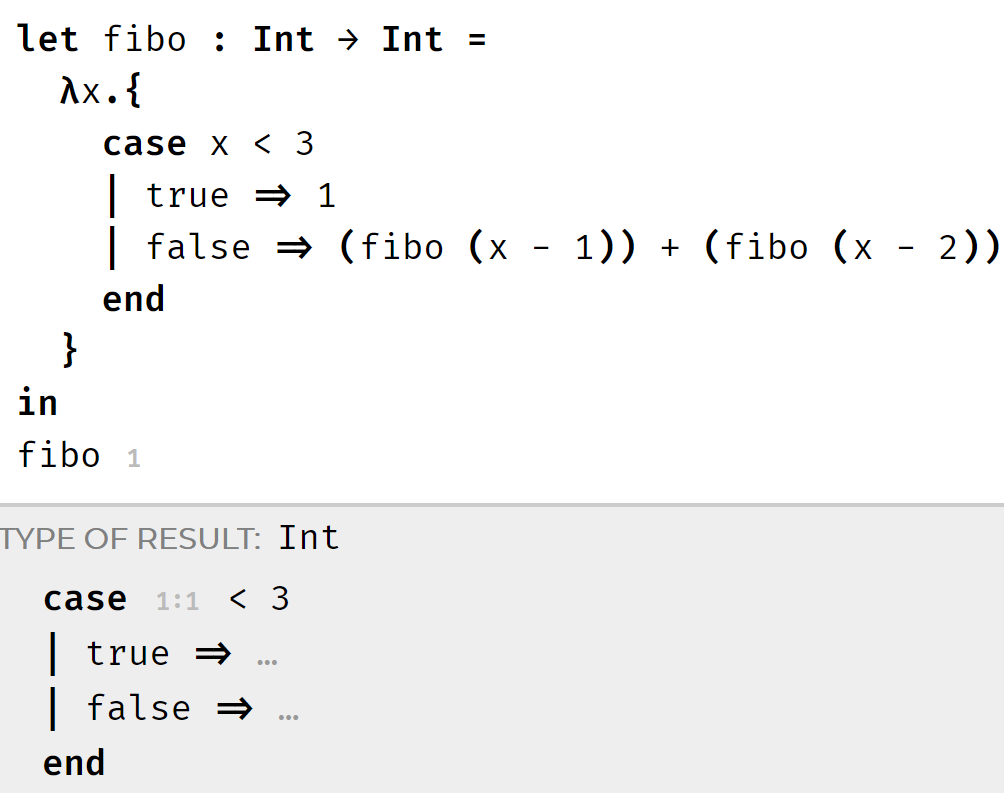
\includegraphics[width=\textwidth]{img/pause_fibo.png}
      \caption{Example of a program with hole as argument}
      \label{fig:pause1}
  \end{subfigure}
  \hfill
  \begin{subfigure}[b]{0.3\textwidth}
    \centering
    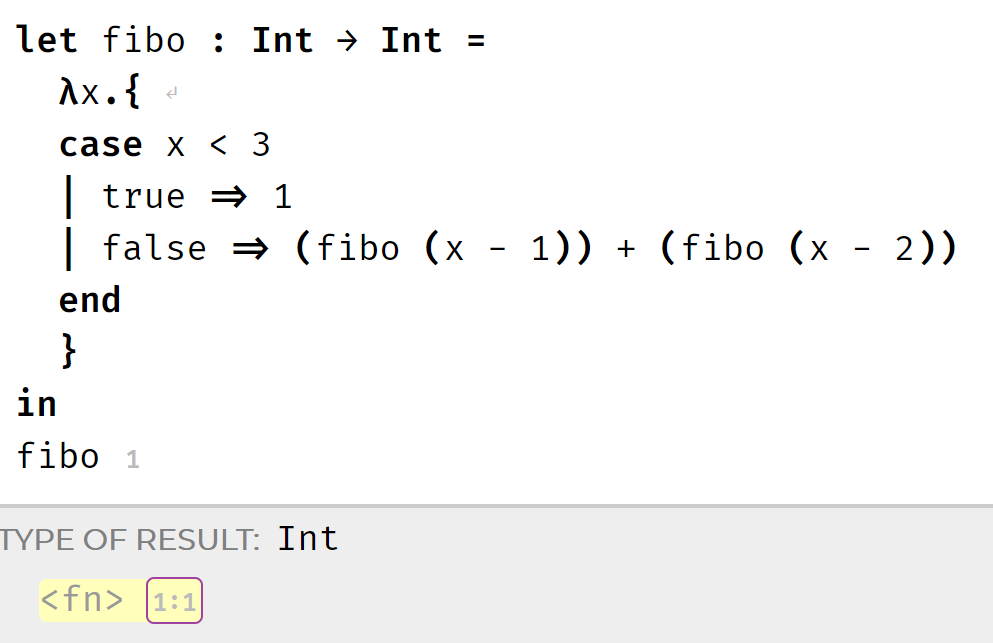
\includegraphics[width=\textwidth]{img/pause_fibo2.png}
    \caption{Example of paused evaluations}
    \label{fig:pause2}
  \end{subfigure}
  \hfill
  \begin{subfigure}[b]{0.3\textwidth}
      \centering
      %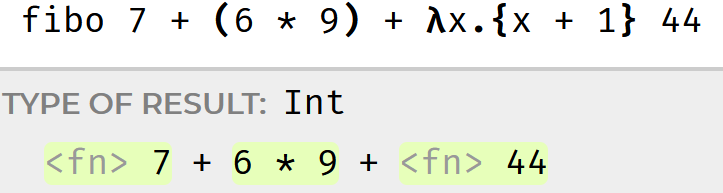
\includegraphics[width=\textwidth]{img/interactive.png}
      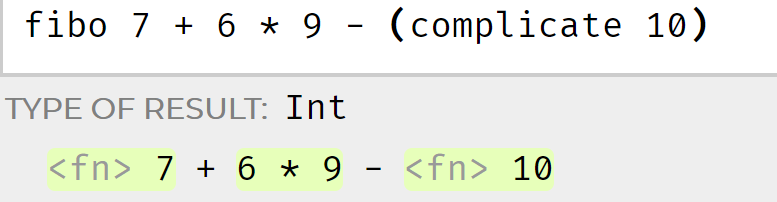
\includegraphics[width=\textwidth]{img/interactive1.png}
      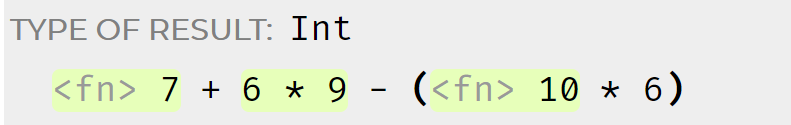
\includegraphics[width=\textwidth]{img/interactive2.png}
      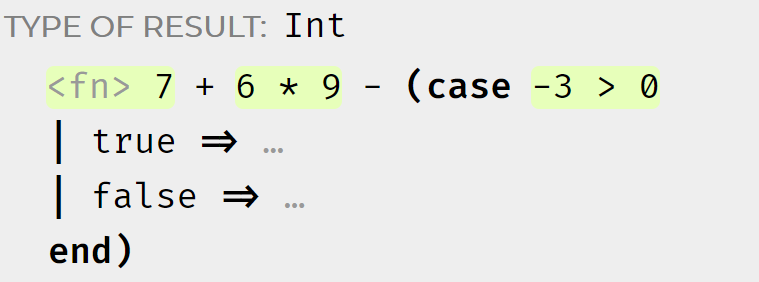
\includegraphics[width=\textwidth]{img/interactive3.png}
      \caption{Example of choosing which active expression to evaluate}
      \label{fig:multiple}
  \end{subfigure}
    \caption{Three programs in \Hazel}
    \label{fig:intro_example}
\end{figure}

% Findler et al.[citation] developed a stepper for DrScheme in their programming environment. Cong and Asai [citation] used the contextual dynamics to build a stepper, which takes subexpression out and plug in after evaluation. In this paper, we will use the similar strategy to develop the stepper. 

Figure \ref{fig:pause1} is an example of expression with a hole. The evaluation result is a case expression with a hole as parameter. However, the origin expression is already simple enough and it is unnecessary to expand like that especially when there are many cases in the function. In \Hazel, evaluation is live. Therefore, this result might arise momentarily so that its size may distract the user. It also reveals internal details about how the function is implemented. Therefore, we want to develop a stepper that can detect this situation so that it will pause until user requires it to step further. The result shown in Figure \ref{fig:pause2} with yellow box is calculated by our stepper with pause judgement.

Figure \ref{fig:multiple} shows an expression with three parts. The left part is heavy since it takes many steps to evaluate. However, user might just want to debug the right complicated part. According to the regular evaluation order for \Hazel, there should be only one way to step for any non-final programs. So, user has to click many times to reduce the left one in order to debug the right one. Our solution is to provide options for user to choose where to step. In the Figure \ref{fig:multiple}, the green boxes contain subexpressions that can be evaluated. In these three results, we always click the right box to evaluate. We can see how the multiple contexts work.

Our interactive stepper is specified by a pausing judgement and a simple algorithm to decompose multiple evaluation contexts. Furthermore, it also has a webview so that user can click boxes to step expressions.

\parahead{Contributions} The contributions of this paper are: (1) a pausing judgement in section ~\ref{sec:pause}; (2) an algorithm to decompose multiple evaluation contexts in section ~\ref{sec:condy}.